\section{A wider, fair test}\label{sec:breadth}
\paragraph{Design.} Seven families: unit squares in a square, a circle and a triangle; unit triangles in a triangle and a square; unit hexagons in a square; and, as a control, unit-diameter circles in a square, where hardening changes nothing because a disk is already a disk. Best known values come from the Squares Project \cite{squaresproject}, Friedman's catalogue \cite{friedmancenter} and Packomania \cite{packomania}; truncated catalogue values (``$2.956+$'') count as reached within their printed precision. All $n$ from 2 to 30 (to 20 for hexagons) are used, \CsevenInstances{} instances in all, minus five reserved for tuning.

Each method was tuned twice, with the same effort: a $3\times3$ grid on held-out instances, scored first by median gap (campaigns C01--C03) and then by the lowest size reached (C06, on harder held-out instances with $n>30$). Each method then ran 32 times per instance with an equal budget of pair evaluations, and the best run of each instance and method was tightened. Every campaign's plan, including its decision rule, was committed before its first run; changes after a campaign started are recorded as amendments.

\paragraph{Result.} Table~\ref{tab:main} counts, per family, the instances on which each method's lowest size is the lowest of all five. Rigid starts reach the lowest size most often overall (\CsevenRigidLowest{} instances, against \CsevenGrowLowest{} for grow and \CsevenHardenLowest{} for harden), and reach the best known value most often (\CsevenRigidSolved{} against \CsevenGrowSolved{} and \CsevenHardenSolved{}). Over instances solved by exactly one of the two, rigid against harden is \CsevenSignRigid{} (one-sided $p=\CsevenSignPRigid$). Simulated annealing improved most from tuning for the lowest point and is competitive on several families; perturbation--compression stays far behind at this budget. No run went below a published value, and \CsevenUnsolved{} instances were solved by no method. The median-tuned comparison (C04, Table~\ref{tab:median} in the appendix) gives the same ordering.

\begin{table}[t]\centering\small
\begin{tabular}{lrccccc}
\toprule
family & $N$ & \textbf{harden} & \textbf{grow} & \textbf{rigid} & \textbf{sa} & \textbf{pc} \\
\midrule
squares in square & 28 & \textbf{27 (5)} & 21 & 23 (1) & 21 & 17 \\
squares in circle & 28 & 16 (6) & \textbf{17 (4)} & 15 (3) & 14 (2) & 8 \\
squares in triangle & 29 & 28 & 27 & \textbf{29} & 24 & 8 \\
triangles in triangle & 28 & 18 & 24 (2) & \textbf{26 (4)} & 19 & 10 \\
triangles in square & 28 & 14 (2) & 17 (3) & \textbf{22 (7)} & 9 & 5 \\
hexagons in square & 18 & 15 & 14 & \textbf{16 (1)} & 14 (2) & 9 \\
circles in square (control) & 29 & \textbf{24} & \textbf{24} & \textbf{24} & \textbf{24 (2)} & 15 (1) \\
\midrule
all & 188 & 142 (13) & 144 (9) & \textbf{155 (16)} & 125 (6) & 72 (1) \\
reached best known & & 125 & 129 & 133 & 115 & 71 \\
\bottomrule
\end{tabular}
\caption{Lowest point by family (C07; every method tuned for its lowest point, 32 runs per instance, matched budget). Each cell: number of instances on which the method\textquotesingle s lowest tightened size is the lowest of all five methods; in brackets, on how many it is the only method that low. Bold: most per family.}
\label{tab:main}
\end{table}


\begin{figure}[t]\centering
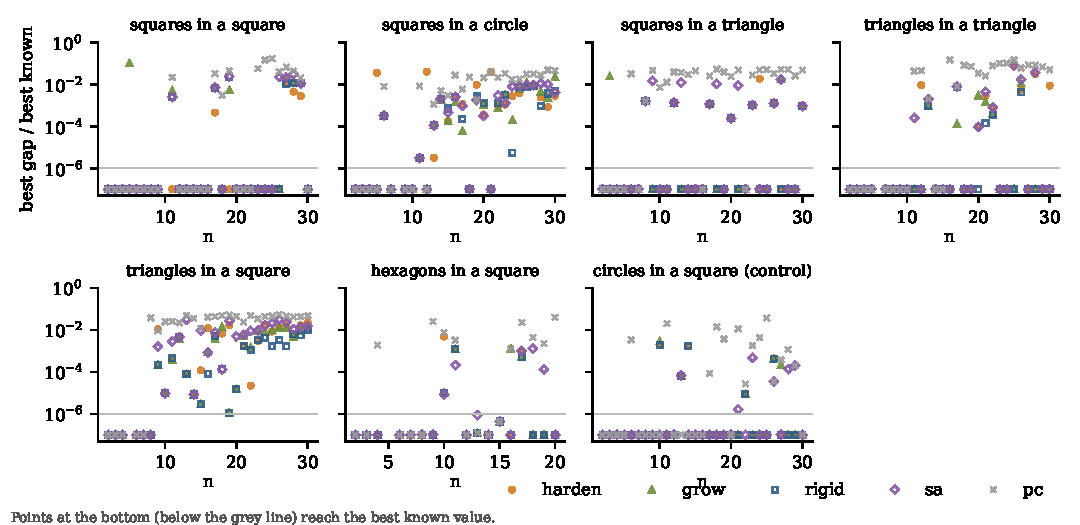
\includegraphics[width=\linewidth]{figures/gaps}
\caption{Lowest size reached per instance, relative to the best known value (C07). Points on the bottom row reach it.}\label{fig:gaps}
\end{figure}
